\chapter{Systemarchitektur des Quadrocopters}
\label{chap:Systemarchitektur}
Zu Beginn wird in diesem Kapitel die Hardwarearchitektur sowie die Kommunikationsstruktur vorgestellt. Ziel ist es einen �berblick der verbauten Sensoren und Recheneinheiten sowie deren Vernetzung untereinander zu erlangen. 
\section{Hardwareaufbau}
\label{sec:Hardwareaufbau}
Zum Einsatz kommt der AscTec Pelican der Firma ASCENDING TECHNOLOGIES. Dieser Quadrocopter ist speziell f�r die Forschung entworfen worden. Seine Turmstruktur erm�glicht eine einfache Integration zus�tzlicher Sensoren und Nutzlasten. Durch diese Flexibilit�t im Aufbau ist es Ziel dieses Teilkapitels einen �berblick zu geben, wo die einzelnen Komponenten positioniert sind. Begleitend zum Text ist der Aufbau in Abbildung \ref{fig:hardwareaufbau} sowie etwas ausf�hrlicher, mit den Daten der Komponenten, im Anhang dargestellt.\\

	\begin{figure}
		\centering
		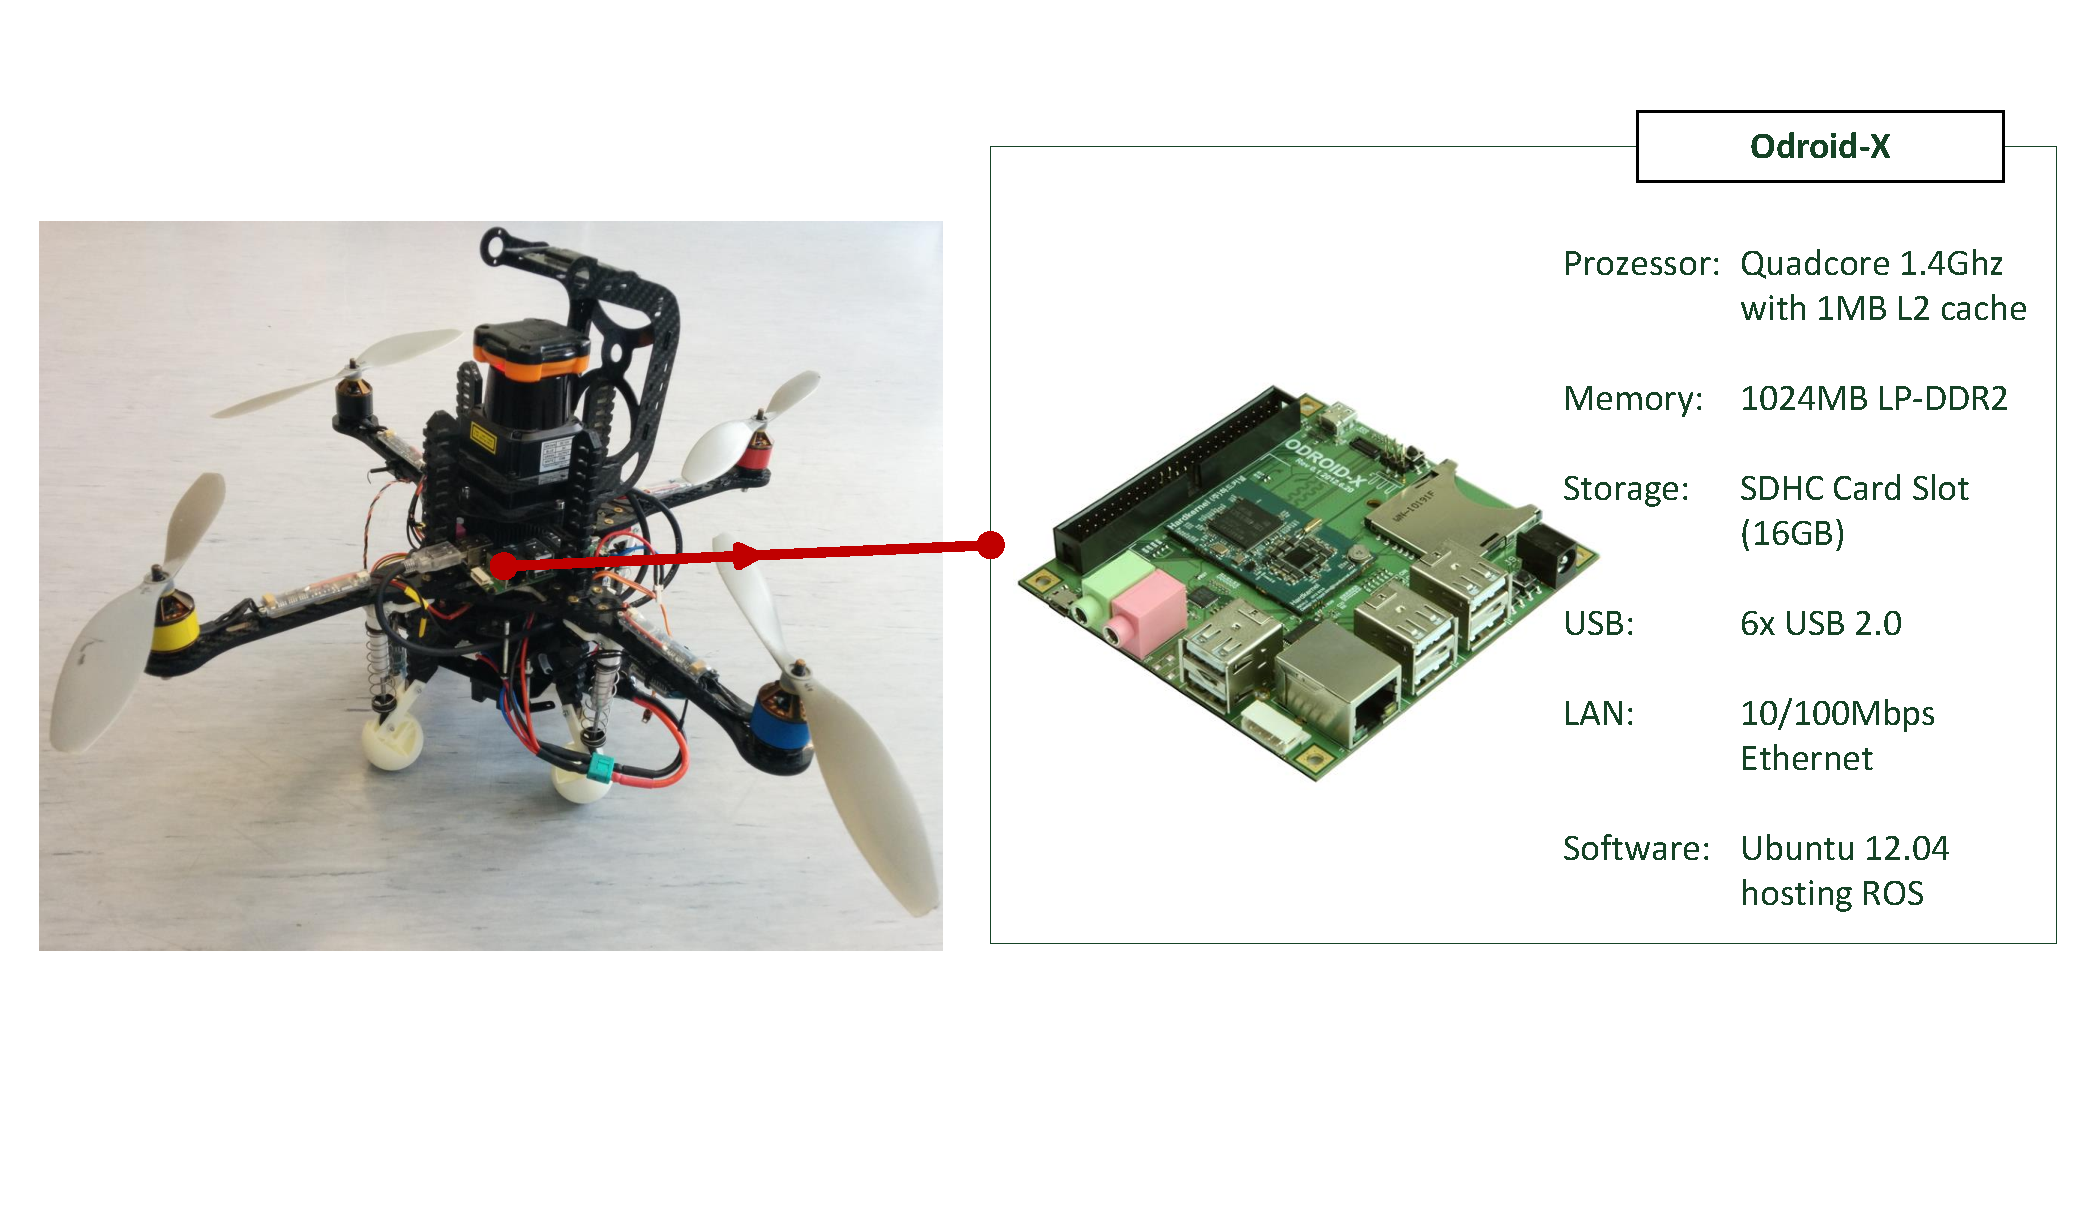
\includegraphics[width = 0.75\textwidth]{images/quad_odroid}
		\caption[Hardwareaufbau]{Hardwareaufbau des Quadrocopters...DIESE GRAFIK IST EIN PLATZHALTER GRAFIK NUR MIT NAMEN DER KOMPONENTEN}
		\label{fig:hardwareaufbau}
	\end{figure}

F�r jeder der vier mit einem Propellor verbundenen Elektromotoren, ist ein separate Motorcontroller zust�ndig. Diese sorgen daf�r, dass sich die von der \gls{FCU} angeforderten Drehzahlen einstellen. 

Die FCU ist die zentrale Steuer- und Regeleinheit des Quadrocopters. Sie besitzt zwei ARM7 Prozessoren, einen \gls{LLP} und einen \gls{HLP}. Au�erdem verschiedene Kommunikationsschnittstellen (vgl. Kapitel \ref{fig:Kommunikationsstruktur}). Zus�tzlich dient sie als inertiale Messeinheit (engl. \gls{IMU}). Diese Einheit wird zur Bewegungsdetektion sowie zur Bestimmung der Lage und Ausrichtung ben�tigt. Sie ist nicht zur Positionsbestimmung in einem ortsfesten Koordinatensystem (Koordinatensysteme siehe Kapitel HIER MUSS EINE REF hin) geeignet. Bestandteile der IMU sind ein 3D-Beschleunigungssensor, drei Drehratensensoren(Gyros), einem Kompass sowie einem Drucksensor zur Ermittlung der Flugh�he anhand des Luftdrucks. Verbaut sind die Sensoren mit Ausnahme des Kompass direkt auf der Platine (siehe Abbildung \ref{fig:fcuplatien}).

	\begin{figure}
		\centering
		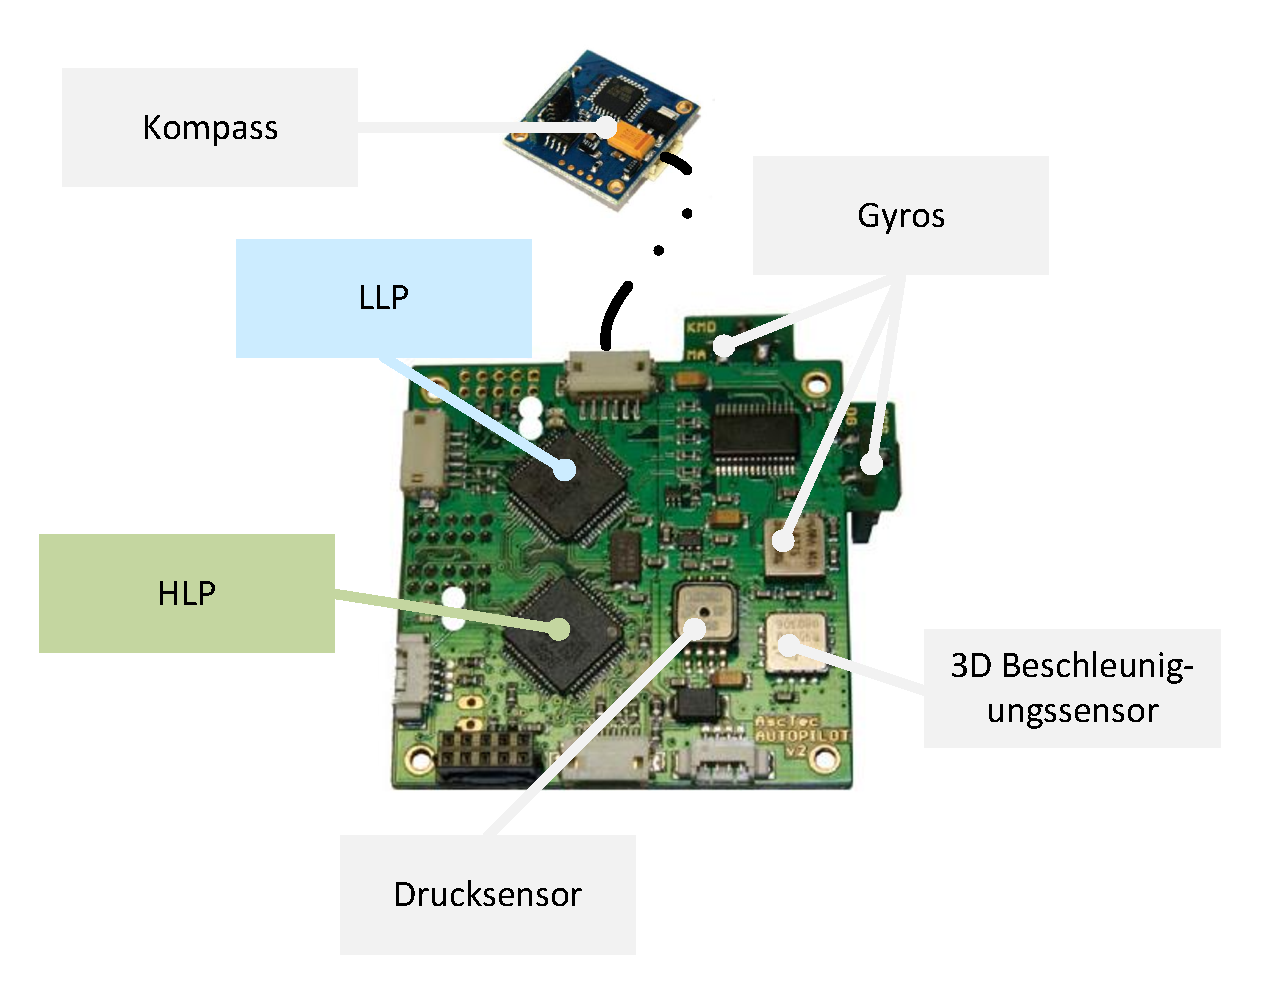
\includegraphics[width = 0.75\textwidth]{images/FCU_Platine}
		\caption[fcuplatine]{Platine der \gls{FCU}}
		\label{fig:fcuplatien}
	\end{figure}

Da der Einsatzbereich im Indoorbereich liegt, ist Drucksensor ist zur H�henbestimmung in geschlossenen R�umen nicht eignet, da er erst ab einer H�he von 5m zuverl�ssige Werte liefert. Daher wurde in einer vorangegangen Arbeit von Jan Kallwies (lITERAURVERWIES JAN) die Hardware um ein Modul zur Messung der H�he im Indoorbereich erweitert. Auf diesem Modul befinden sich ein zwei Infrarotsensoren f�r den Nahbereich. Diese decken, aufgrund der Einbauh�he, den Bereich von 0 cm bis 146 ab. Erweitert wird der Messbereich durch einen Ultraschallsensor f�r Entfernungen von bis zu 5 m. Aus diesen drei Sensordaten wird �ber einen Extended-Kalman-Filter die Flugh�he bestimmt. Eine genaue Beschreibung dieses Fusionsfilters kann in der Arbeit von Jan Kallwies [LITERATURVERZEICHNIS] nachgelesen werden. Da in dieser Arbeit die Navigation in der horizontale Ebene den Schwerpunkt darstellt, wird dieses Modul nicht weiter behandelt.


Um allerdings in der Horizontalen navigieren zu k�nnen, muss die Position des Flugk�rpers in der x-y Ebene (VGL kOORDINATENSYSTEME) bekannt sein. Da dies, wie schon beschrieben, nicht mit der Inertialsenorik m�glich ist, wurde in die Turmstruktur der Laserscanner UTM-30LX der Firma Hokuyo integriert. Dieser Scanner hat eine maximale Reichweite von 30 m und Abtastbereich von 270�. Die Umlaufdauer betr�gt dabei 40 Hz, d.h. alle 25 ms wird ein neuer Umgebungssan zur Verf�gung gestellt.    

Damit zur Berechnung der Position sowie Implementierung weiterer Algorithmen und Funktionen ausreichend Rechenleistung vorhanden ist, befindet sich auf dem Quadrocopter ein zus�tzlicher Odroid-X Mikrocomputer mit einem Quad Core Prozessor mit 1.4 Ghz und einen 1024MB LP-DDR2 Arbeitsspeicher. Au�erdem befinden sich auf dieser Entwicklungsplattform  sechs USB-Anschl�sse sowie ein 10/100Mbps Ethernet-Anschluss.\\


Nun sollte man einen �berblick �ber die im Quadrocopter verbauten Komponenten besitzen. Wie die Einheiten untereinander vernetzt sind, darauf wird im folgenden Kapitel \ref{sec:Kommunikationsarchitekur} eingegangen.

     

%In der Grundausstattung enthalten ist das AutoPilot Board auch \gls{FCU}  genannt. Diese Board ist die Steuer- und Regeleinheit des \gls{UAV}, zu deutsch \glqq unbemanntes Luftfahrzeug \grqq. Die Inertialsensorik befindet sich ebenfalls auf dieser Platine. Diese beinhaltet einen Beschleunigungssensor, einen Lagesensor sowie einen Drucksensor zur H�henbestimmung.



 %Wie sich aus dem Name schlie�en l�sst ist diese Einheit zur Steuerung und Regelung des \gls{UAV}, zu deutsch unbemanntes Luftfahrzeug. 
%Darauf integriert sind die Inertialsensoren wie Beschleunigungssensor, Lagesensor(Gyro), Kompass und Drucksensor. 




\section{Kommunikationsstruktur}
\label{sec:Kommunikationsarchitekur}

Nachdem im vorigen Kapitel \ref{sec:Hardwareaufbau} der Hardwareaufbau des Flugobjekts vorgestellt wurde, geht es in diesem Teilkapitel um 

die Kommunikationsstruktur und Verwendungszwecke der Hardwarekomponenten.  


\begin{figure}
	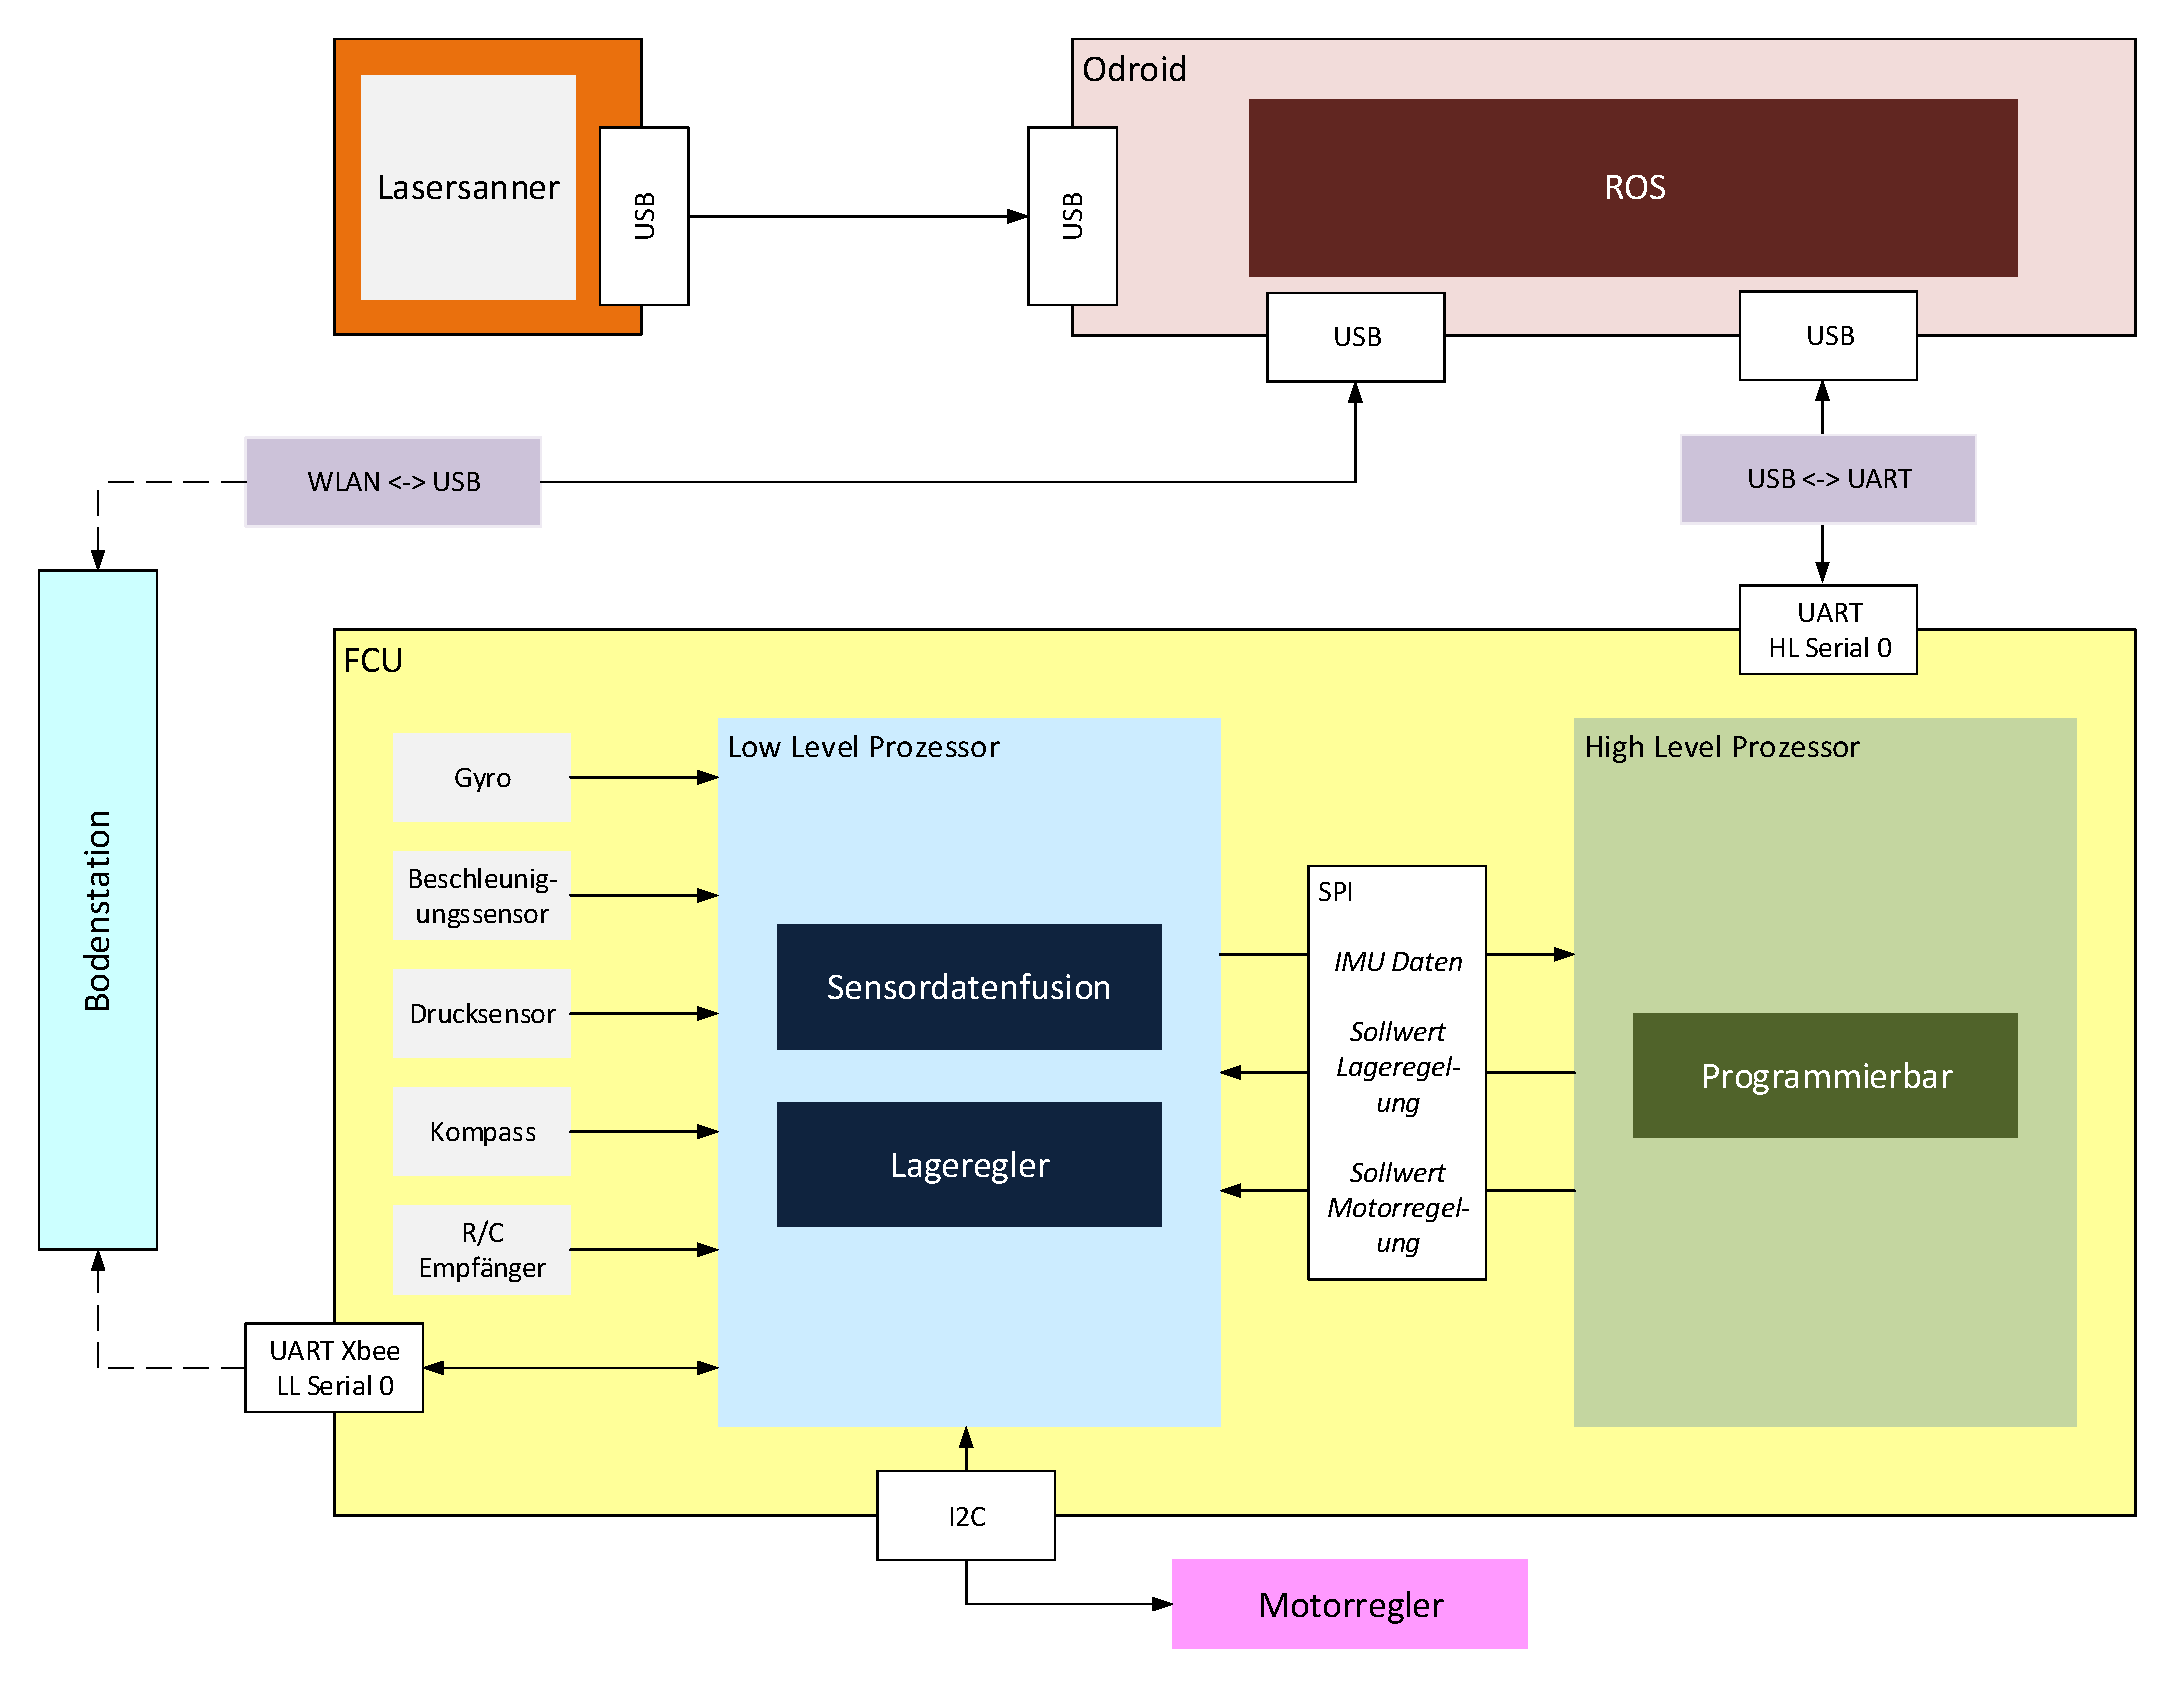
\includegraphics[width = \textwidth]{images/Kommunikationsarchitektur}
		\caption[Kommunikationsstruktur]{Kommunikationsstruktur des Quadrocopters  In Grafik fehlt das Modul zur H�henmessung Kompass auf deutsch}
		\label{fig:Kommunikationsstruktur}
\end{figure}
